%(BEGIN_QUESTION)
% Copyright 2011, Tony R. Kuphaldt, released under the Creative Commons Attribution License (v 1.0)
% This means you may do almost anything with this work of mine, so long as you give me proper credit

En operatør ber deg komme til et DCS-bilde for å vise trenden til en ``syklende'' sløyfe. Din første diagnostiske test er å sette sløyferegulatoren i manuell modus. Resultatet før og etter overgang fra auto til manuell modus vises i denne trenden:

$$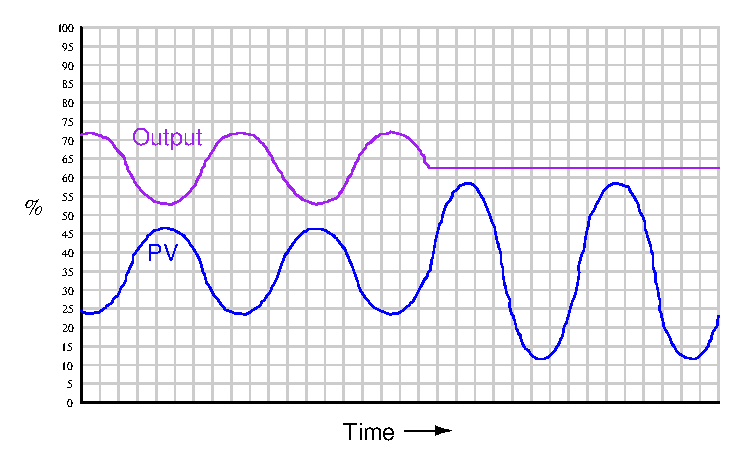
\includegraphics[width=15.5cm]{i01648x01.eps}$$

Resultatet av å sette regulatoren i manuell modus overrasker deg -- om noe, forventet du at PV skulle ``roe seg'' heller enn å bli {\it mer} syklisk! Avgør hva denne trenden forteller oss om typen syklingsproblem og mulige årsaker. Forklar også hvorfor det var en god diagnostisk idé å sette regulatoren i manuell modus.

\vskip 10pt

Hvis du var instrumentteknikeren som oppdaget dette, hva ville vært neste diagnostiske steg?

\vskip 20pt \vbox{\hrule \hbox{\strut \vrule{} {\bf Forslag til sokratisk diskusjon} \vrule} \hrule}

\begin{itemize}
\item{} Generelt forteller en pen, {\it sinusformet} oscillasjon oss noe spesifikt om årsaken til oscillasjonen. Hva antyder sinusformen for oss?
\item{} Basert på denne trendgrafen, kan vi avgjøre om regulatoren er direkte- eller reversvirkende? Hvis ja, hvilken virkemåte er det?
\item{} Basert på denne trendgrafen, kan vi identifisere dominerende reguleringsvirkning (P, I eller D) i regulatoren? Hvis ja, identifiser hvilken virkning som gjør mest av arbeidet her.
\item{} Basert på denne trendgrafen, kan vi identifisere hvor mye forsterkning (P-virkning) som er programmert i regulatoren? Hvis ja, anslå regulatorens forsterkningsverdi.
\item{} Basert på denne trendgrafen, kan vi identifisere prosessforsterkningen? Hvis ja, anslå prosessforsterkningen.
\end{itemize}

\underbar{file i01648}
%(END_QUESTION)





%(BEGIN_ANSWER)

Uansett hva problemet er, ligger det {\it ikke} i denne sløyferegulatoren!

%(END_ANSWER)





%(BEGIN_NOTES)

At syklingen blir verre når regulatoren settes i manuell modus forteller oss at syklingen kommer fra noe annet enn regulatoren, og ikke at regulatoren selv er årsaken. Det mest sannsynlige er at en {\it annen} reguleringssløyfe i det større systemet sykler, og påfører denne regulatoren en syklisk {\it last} som den ikke klarer å nøytralisere i automatisk modus. Dette er hva sinusformen antyder: en overinnstilt regulator som oscillerer ved sin ultimate periode (frekvens).

Det er mulig at situasjonen kunne forbedres ved å øke aggressiviteten i denne regulatoren, slik at den reagerer raskere og mer effektivt på sinuslasten, men hovedårsaken til problemet er definitivt noe annet i prosessen som oscillerer.

%INDEX% Process troubleshooting: diagnosing problem via trend recording

%(END_NOTES)
